\chapter{Authenticating People}


\section{Authentication}
In this class, we will talk a lot about requests
going to a computer system.
And a lot of security comes down to looking at that request and deciding
how to handle it.
For this, it is crucial to know
\textit{who} issued the request. Then, we can
decide whether the class should be allowed.

Typically, a computer system performs two steps before processing
a request:
\begin{enumerate}
  \item \textbf{Authenticate:} Identify the person or machine (the ``\emph{principal}'') making the request.
  \item \textbf{Authorize:} Decide if the principal is authorized to make the request.
\end{enumerate}

\section{Passwords}
Passwords are the most widespread method 
that humans use to authenticate to computer systems.
We use passwords to authenticate to ATMs,
our phones, our computers, and so on.

Examples of human-chosen passwords are:
\begin{itemize}
	\item \ttt{password}
	\item \ttt{PaSsW0rd1!}
	\item \ttt{purple-student-hat}
\end{itemize}

Which of these passwords are ``good'' and which
are ``bad?''
Many sites would let you use
\ttt{PaSsW0rd1!} as your password but would not allow
you to use \ttt{purple-student-hat}.
However, what really matters is the adversary's
uncertainty about your password.
That is, what we really care about is that the adversary
will not be able to guess your password in
a small number of guesses.

%And most likely, they will guess the
%most common passwords first.

\begin{figure}
  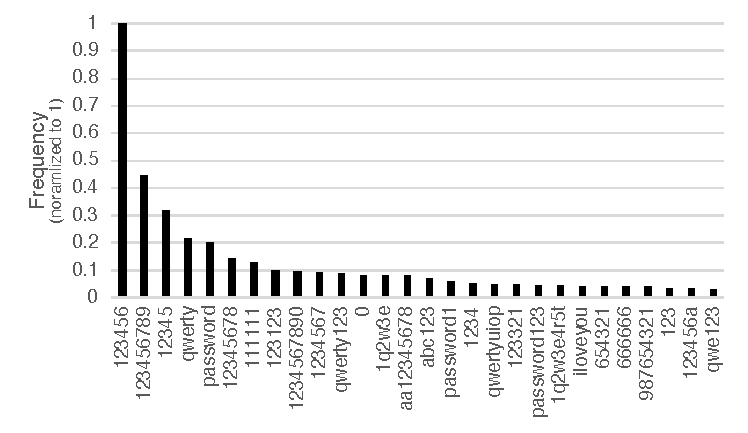
\includegraphics[width=\textwidth]{figs/password-dist.pdf}
  \caption{The most common passwords, according to
  NordPass (\url{https://nordpass.com/most-common-passwords-list/}),
  sorted by their frequency descending.
  A small number of common passwords dominate.
  \todo{Fix the $y$-axis here.}}
\end{figure}

Ideally, we would want all passwords to be equally as likely,
from the adversary's perspective.
But that is not the case.
People have to remember their passwords,
and it turns out that many people are likely to choose the same password.

\marginnote[-2in]{
  \begin{tabular}{cc}
    Rank & Password \\
1 & \ttt{123456}\\
2 & \ttt{123456789}\\
    3 & 12345\\
    4 & qwerty\\
    5& password\\
    6& 12345678\\
    7& 111111\\
    8& 123123\\
    9& 1234567890\\
    10& 1234567\\
    11& qwerty123\\
    12& 000000\\
    13& 1q2w3e\\
    14& aa12345678\\
    15& abc123\\
    16& password1\\
    17& 1234\\
    18& qwertyuiop\\
    19& 123321\\
    20& password123
  \end{tabular}
  \medskip
  \captionof{table}{The most popular passwords in 2021, according to 
  NordPass, \url{https://nordpass.com/most-common-passwords-list/}.}
}

How do we convince humans to choose hard-to-guess passwords? 

\begin{itemize}
  \item \emph{Require longer passwords?} If someone tries to use 
    \ttt{abc123} as a password but it's not long
    enough, they might use \ttt{abc123456}---but
    this doesn't really add much uncertainty.
    There are standard ways to lengthen passwords,
    and a clever attacker will try these first.
  \item \emph{Prohibit using common English words in passwords?}
    It's not clear that this is a good idea.
    Five randomly chosen words from the dictionary will
    form a strong password, and prohibiting English words
    in passwords may make passwords much more difficult to remember.
      
  \item \emph{Force password changes?}
    This makes it harder for users to remember their password, and
    may actually cause users to choose easier-to-guess passwords
    (since these may be easier to remember).
    Forcing a password change may be more effective if the system has
    suffered a breach and the users' passwords have leaked out.

  \item \emph{Generate password for the user?} This is the only way
    to be guaranteed a strong password. But then the user is stuck
    having to memorize a random string.
    Few systems take this approach, mostly because it is so inconvenient
    for the system's users.

\end{itemize}

So, in spite of our best efforts, users will likely choose
easy-to-guess passwords.
What can we do about this?

\subsection{Dealing with poor passwords}
A ``good'' password might be sampled from a distribution with roughly
20 bits of \marginnote{\emph{Entropy} is a
way to quantify the adversary's uncertainty about
a value sampled using a random process, or from a particular probability distribution.
If a distribution has $b$ bits of entropy, then
it will take at least roughly $2^b$ guesses for an attacker to correctly
guess a value sampled from this distribution.

The uniform distribution over 128-bit strings has 128 bits of entropy.
The distribution from which humans typically choose their passwords
has much less entropy---empirically, more like 20 bits.}
entropy---if an adversary is able to make $2^{20}$ guesses
at the password, they can expect to guess the password correctly.
And with current technology, guessing $2^{20}$ times is easy.
So when using passwords as an authentication mechanism,
we must find a way to limit guesses. 

A standard way to deal with the fact that passwords are easily
guessable is to limit the number of guesses an attacker gets
at the password.
For example, some phones allow 10 guesses at the screen-lock PIN 
before the device resets itself.
Limiting the number of guesses effectively prevents a \emph{single}
account from being compromised---provided that the password is not
too too weak.
One downside is guess limits create the possibility for denial-of-service
attacks: an attacker can potentially make 10 guesses at your password and lock
you out of your phone or online-banking account.

In addition, in many physical computer systems have multiple authorized 
users, each with their own password.
If the guess limit is enforced only on a per-user basis, then an attacker
can often compromise \emph{some} account on the machine if it is allowed
10 guesses at \emph{every} user's password.
Preventing these types of attacks requires some additional measures: websites
that use password authentication rate-limit guesses by IP, or use CAPTCHAs, etc.

\subsection{Storing Passwords}

\iffalse
The most obvious way to store passwords on
a server would be to just store each username
along with their password.

\begin{tabular}{c|c}
	user & password \\
	\hline
	alice & \ttt{abc123} \\
	bob & \ttt{1234} \\
\end{tabular}

\textbf{Risk}: adversary steals the password table (by breaking in to the system, stealing the hard drive, etc). Now, every user's account is compromised. However, since many users use the same password across many sites, those other sites are now compromised too.

So, it would be great if we could check whether a user's inputted password is correct without storing the actual password. To do this, we can use a \textit{hash function}. For our current purposes, a hash function is a deterministic way of scrambling the input such that it cannot easily be reversed. That is, the same input will always produce the same output, but given an output there is no easy way to determine the corresponding input.

\begin{tabular}{c|c}
  user & $H(\text{pw})$ \\
	\hline
	alice & $h_a$ \\
	bob & $h_b$ \\
\end{tabular}

Now, if the database gets compromised, only the \textit{hashes} of those passwords are made public. Assuming we choose a \textit{one-way} hash function, meaning that there is no easy way to compute $pw$ given only $H(pw)$, the only way to find $pw$ and log into the user's account then is to figure out the mapping from each possible password to H(pw) and find the one that matches. 

To make this more difficult, systems can make use of an expensive $H$ function. These are often called Key Derivation Functions to separate them from hashes that are meant to be fast. Examples are bcrypt and scrypt. In effect, stealing the database removes any rate limiting that is enforced by the server. But we can add cryptographic rate limiting by using a KDF to generate the hash.

However, if all systems use the same hash function (hash functions are hard to make, so they are likely to), then many adversaries could get together and compute a \textit{rainbow table} that maps $H(pw)$ to $pw$. 

\subsection{Avoiding pre-computation: salting}
\fi

Since, as we have seen, passwords are easy to guess, avoiding 
password-based authentication entirely is the safest option where
possible.

When a system must use passwords for authentication, the safest
way to store them (e.g., on a server) is using an 
\emph{salted cryptographic password-hashing function}.
The goal is to make it as difficult as possible for an attacker
to recover the plaintext passwords, given the hashed values stored on the server.

To describe how this works: when a user creates an account with password pw,
the server chooses a random 128-bit string, called a \emph{salt},
and the server stores the salt and the hash value
$h=H(\text{salt}\|\text{pw})$, where $H$ is a special password-hashing function.

The server then stores a table that looks like this:

\medskip
\begin{tabular}{c|c|c}
  user & salt & $H(\text{salt}\|\text{pw})$ \\
	\hline
	alice & $r_a$ & $h_a$ \\
	bob & $r_a$ & $h_b$ \\
\end{tabular}
\medskip

Later on, when the user sends a password $\text{pw}'$ to the server to authenticate, 
the server can use the salt and hash function to compute a value $h' = H(\text{salt}\|\text{pw}')$.
If this hash value $h'$ matches the server's stored value $h$ for this user,
the server accepts the password.

To explain the rationale for this design:
\begin{itemize}
  \item The password-hashing function $H$ is designed to be relatively expensive
        to compute---possibly using a large amount of RAM and taking a second or 
        more of computation.
        This makes it more difficult for an attacker to brute-force invert the
        hash value, since each guess at the password requires a second of computation
        (instead of the microseconds required to compute a standard hash function,
        such as SHA256).
  \item The use of a per-user random salt ensures that guesses at one user's password
        are useless in inverting another user's password hash.
        Salting also defeats \emph{precomputation attacks}, in which an attacker
        precomputes the hashes of many common passwords to speed up this hash-inversion
        step later on.
\end{itemize}


\section{Authentication over the Network}
We have so far been talking about a human manually
authenticating to a device (ATM, phone, laptop, etc.)
by physically entering a PIN or password into the device.
But we often log in to some server on the network---Facebook,
Gmail, MIT, and so on. 
In this scenario, we can get much more creative
with the authentication mechanism we use and the
security properties we can demand.

\subsection{Password Manager}
When using passwords to authenticate to a website, 
a user can install a password manager on their
computer that will generate random passwords for them.
Since the user doesn't need to remember these passwords,
they can be sampled truly at random from a high-entropy distribution.
Once the user logs into their computer, they can
then access their randomly generated passwords and
use them to log in to their websites. 

Internally, the password-manager software maintains a table of 
servers and the corresponding passwords:

\medskip
\begin{tabular}{c|c|c}
  server & user & pw \\ \hline
  \ttt{amazon.com} & \ttt{alice} & \ttt{3xyt42...} \\
  \ttt{mit.edu} & \ttt{alice4} & \ttt{a21\$z...} \\
\end{tabular}
\medskip

But password-based authentication, even with a strong password,
still requires sending passwords over the network.
If an adversary can watch our network, they can see our password.
Transport-later security, which we will discuss later on, can
protect against network eavesdroppers, but a better solution is to
authenticate without ever sending the password over the network.

\subsection{Challenge-Response Protocols}
We now assume that our computer has some key~$k$
(e.g., a random 128-bit string), 
and the server also holds the same key~$k$. 
Then a challenge-response protocol proceeds as follows:

\todo{use the crypto latex library to make this nice}

\begin{enumerate}
	\item The server chooses a long random string~$r$, which we often call a \textit{nonce} and sends it to the authenticating client.
  \item The client computes an authentication ``tag'' $t \gets \MAC(k, r)$, where $\MAC(\cdot, r)$ is hard to compute without knowing $k$.
    (The function $\MAC$ here is a Message Authentication Code, which we will talk more specifically about
        in \cref{lec:mac}.)
        The sends the MAC tag $t$ to the server.
  \item The server receives a tag $t'$ from the client and ensures that $t' = \MAC(k,r)$.
        If so, the server considers the authentication successful.
\end{enumerate}

\marginnote{An \textbf{unsafe} way for the client to simultaneously authenticate to the 
server and send a request would be for the client to compute the MAC tag $t \gets \MAC(k,r)$
and then send $(t, \mathsf{req})$ to the server.
A network attacker could modify the client's request to $(t, \mathsf{req'})$ en
route to the server without the server being able to detect this attack.}
In practice, the client often wants to simultaneously authenticate to the server
and send a request $\mathsf{req}$, such as $\mathsf{req} = \ttt{rm file.txt}$.
To accomplish this, the client can compute the MAC tag $t$ as
$t_{\mathsf{req}} \gets \MAC(k, r \| \mathsf{req})$.,
Then the client sends the pair $(t_{\mathsf{req}}, \mathsf{req})$ to the server.
In this way, the server can simultaneously authenticate the client
and be sure that the request $\mathsf{req}$ came from the client.

\section{Two-Factor Authentication}
As we have already seen, passwords are a weak authentication
mechanism: humans are bad at choosing strong passwords and 
attackers have become good at stealing password databases
and recovering many users' passwords at once.

A common technique to harden password-based authentication systems
is to combine passwords with a second method of 
authentication---one with a different failure mode. 
Common authentication schemes are:

\begin{itemize}
	\item Something you know: password, PIN, etc
	\item Something you have: USB key, phone, etc
	\item Something you are: biometrics (fingerprint, face ID)...
\end{itemize}

\subsection{Time-based One-Time Passwords (TOTP)}
In this scenario, the server requests a code along
with the password. The user has a device, such as 
a phone, that shares a secret key $k$ (e.g., a random 128-bit string) 
with the server.
Both parties agree on a protocol by which to
generate this code---something like $\MAC(k, \texttt{gettimeofday() / 30})$.
The phone can generate the code, display it to the user, and the server
can then verify the code by recomputing it.

\textbf{A common attack.}\marginnote{A \emph{phishing} attack is one
in which an attacker tricks a user into giving away their Gmail password,
for example, by creating a website that looks, for example, like the \ttt{gmail.com}
login page.}
Time-based one-time passwords are also an imperfect authentication mechanism.
For example, an attacker can simply ask the user to give her the one-time code by pretend to be tech support, 
or the user's employer, or a customer-service representative.
This is essentially a phishing attack.
The code is then good for 30 seconds, so the attacker can then
just enter the code into the website on their end.
Similar attacks would include setting up a fake
website that looks like the real one, etc.
One benefit of TOTP codes (unlike passwords) is that the attacker
must use a stolen TOTP code within $\approx$30 seconds of stealing
it, which requires a much more sophisticated attack.

\subsection{Avoiding phishing: U2F (simplified)}
To prevent phishing attacks entirely, we can use a more complex authentication protocol.
If we include the name of the server that the user is trying to log in to in the request that we sent to the device,
the code will be bound to a particular website.
For example, the code might look something like $\MAC(k, r\|\ttt{amazon.com})$.
U2F key fobs use a protocol along these lines for authentication.
If the attacker sets up \ttt{amason.com} and gets the user to visit it,
the U2F device will only generate a code that is good for \ttt{amason.com}
and not the real \ttt{amazon.com}. 
	
\section{Biometrics}
Biometrics are physical features like your fingerprints, your face, etc.
They are very convenient to use for authentication, since you will not forget them and cannot easily lose them.
Biometrics are most useful when authenticating in person to a device, such as for phone unlock, or
to grant a person access to a secure vault.
In these settings, the device performing the authentication has a ``trusted input path''
that can provide some assurance that a real human who owns that biometric is on the other end.
Biometrics are not so useful for authenticating over a network because the network typically
does not provide a trusted input path (i.e., does not provide any assurance that the biometric
readings are coming from a real human), and the biometric data itself is not particularly secret.
In particular, if we used biometrics for network authentication,
an adversary who knows what your fingerprints looks like could log in to your account.
(Since biometrics are essentially impossible to change, this is a major drawback.)
